	% !TeX program = lualatex
	% !Mode:: "TeX:UTF-8"
	\documentclass[a4paper]{article}
	
	\usepackage[a4paper,left=1.0in,right=1.0in]{geometry}
	\usepackage{fontspec}
	
	\newfontfamily\myfont[]{Futura Light BT}
	
	\usepackage{tabularx}
	\usepackage{enumitem}
	\usepackage{graphicx}
	\usepackage{float}
	\usepackage{makeidx}
	\usepackage[stable]{footmisc}
	
	%\usepackage[latin1]{inputenc}
	\usepackage{palatino}
	\usepackage{color}
	\usepackage{hyperref}
	\usepackage[german]{babel}
	\usepackage{tikz}
	\usepackage{adjustbox}
	\usepackage{booktabs}
	\newcommand{\tabitem}{~~\llap{\textbullet}~~}
	
	\usetikzlibrary{calc,trees,positioning,arrows,chains,shapes.geometric,%
		decorations.pathreplacing,decorations.pathmorphing,shapes,%
		matrix,shapes.symbols}
	
	\newenvironment*{dummyenv}{}{}
	
	
	\tikzset{
		>=stealth',
		punktchain/.style={
			rectangle, 
			rounded corners, 
			% fill=black!10,
			draw=black, very thick,
			text width=10em, 
			minimum height=3em, 
			text centered, 
			on chain},
		line/.style={draw, thick, <-},
		element/.style={
			tape,
			top color=white,
			bottom color=blue!50!black!60!,
			minimum width=8em,
			draw=blue!40!black!90, very thick,
			text width=10em, 
			minimum height=3.5em, 
			text centered, 
			on chain},
		every join/.style={->, thick,shorten >=1pt},
		decoration={brace},
		tuborg/.style={decorate},
		tubnode/.style={midway, right=2pt},
	}
	
	\hypersetup{
		colorlinks=true,
		linkcolor=black,
		filecolor=magenta,
		urlcolor=cyan
	}
	
	%% a point to check
	\definecolor{checkcolor}{rgb}{0.75, 0.75, 0.75}
	\newsavebox{\definitionbox}
	\newenvironment{checkit}{%
		\begin{lrbox}{\definitionbox}
			\begin{minipage}[t]{0.85\textwidth}%
			}%
			{\end{minipage}\end{lrbox}%
		\begin{center}{\colorbox{checkcolor}{\usebox{\definitionbox}}}%
		\end{center}}
	
	
	
	\title{Einführung in die Wirtschaftsinformatik Zusammenfassung}
	
	\author{K.M et S.F}
	
	\date{2017}
	
	
	
	\begin{document}
		
		{\myfont \maketitle}
			{\myfont \begin{checkit}
				Folgende Zusammenfassung ersetzt weder die Vorlesung noch Übungen, sondern dient als Lernhilfe zur Vorbereitung für die Klausur (Einführung in die Wirtschaftsinformatik). Es gibt keine Garantie auf Vollständigkeit und Richtigkeit dieses Dokuments.
			\end{checkit}
		}
			\pagebreak
			{\myfont \tableofcontents}
			\pagebreak
			
			%\addcontentsline{toc}{section}{Lerneinheit 1}
			\section{Lerneinheit 1}
			\subsection{Lernziele}
			\begin{enumerate}
				%%there has to be a better to solve this italics thing
				\item \hyperref[le1-1]{\textit{Sie erkennen die Bedeutung der Wirtschaftsinformatik.}}
				\item \hyperref[le1-2]{\textit{Sie kennen die Paradigmen und Teilgebiete der Wirtschaftsinformatik.}}
				\item \hyperref[le1-3]{\textit{Sie erhalten Einblick in das Berufsfeld Wirtschaftsinformatik.}}
				\item \hyperref[le1-4]{\textit{Sie kennen die Bedeutung der Ressource Information und von Informationssystemen für Unternehmen.}}
				\item \hyperref[le1-5]{\textit{Sie kennen die Bestandteile und Eigenschaften von Informationssystemen.}}
				\item \hyperref[le1-6]{\textit{Sie können die verschiedenen Arten von Informationssystemen systematisieren.}}
			\end{enumerate}
			
			\subsection{Frage 1}
			\label{le1-1}
			\begin{itemize}
				\item \textbf{Gegenstand} der Wirtschaftsinformatik sind Informations- und Kommunikationssysteme in Wirtschaft und Verwaltung.
				\item \textbf{Ziel} ist die optimale Bereitstellung von Information und Kommunikation nach wirtschaftlichen Kriterien
			\end{itemize}
			
			\subsection{Frage 2}
			\label{le1-2}
			\begin{itemize}
				\item \textbf{Modellierung} $\rightarrow$ Reduzierung der Komplexität
				\item \textbf{Integrationswissenschaft} $\rightarrow$ Zusammenhänge Menschen-Organisation-IKT
				\item \textbf{Gestaltung} $\rightarrow$ betrieblicher Informationssysteme
			\end{itemize}
			
			\subsection{Frage 3}
			\label{le1-3}
			\begin{enumerate}
				\item Hardware die für \textbf{Systeme} benötigt werden
				\item Kosten-Nutzen-Analyse für das geplante \textbf{System} 
				\item \textbf{System}einführung gestalteten
				\item Entscheidung zwischen Standardsoftware und speziell entwickelte Software
			\end{enumerate}
			
			\subsection{Frage 4}
			\label{le1-4}
			%% SOURCE OF THIS SORCERY I JUST DO THE EDIT http://www.texample.net/tikz/examples/assignment-structure/
			\subsubsection{Zeichen, Daten, Information und Wissen}
			\begin{center}
				\begin{tikzpicture}
				[node distance=.8cm,
				start chain=going above,]
				\node[punktchain, draw=none](woop){}; %%nice little hack
				\node (asym) [punktchain ]  {Zeichen};
				\node[punktchain, join,] (disk) {Daten};
				\node[punktchain, join,] (makro) {Information};
				\node[punktchain, join] (konk) {Wissen};
				
				
				%% No. 2
				\draw[tuborg, decoration={brace}] let \p1=(disk.north), \p2=(makro.south) in	
				($(2, \y1)$) -- ($(2, \y2)$) node[tubnode] {KONTEXT};
				
				\draw[tuborg, decoration={brace}] let \p1=(asym.north), \p2=(disk.south) in ($(2, \y1)$) -- ($(2, \y2)$) node[tubnode] {SYNTAX};
				
				\draw[tuborg, decoration={brace}] let \p1=(makro.north), \p2=(konk.south) in ($(2, \y1)$) -- ($(2, \y2)$) node[tubnode] {VERNETZUNG};
				
				\draw[tuborg, decoration={brace}] let \p1=(woop.north), \p2=(asym.south) in ($(2, \y1)$) -- ($(2, \y2)$) node[tubnode] {ZEICHENVORRAT};
				
				\end{tikzpicture}
			\end{center}
			\hrulefill
			\subsubsection{Informationssystem}
			%\textbf{Informationssystem}:
			\begin{quote}
				Es handelt sich um soziotechnische Systeme, die menschliche und maschinelle Komponenten als Aufgabenträger umfassen, die voneinander abhängig sind, ineinandergreifen und oder zusammenwirken.
			\end{quote}
			\hrulefill
			\subsubsection{Information als Wirtschaftsgut}
			%\hrulefill \\
			\begin{quote}
				Um Information als Wirtschaftsgut anzusehen muss eine relative Knappheit bestehen und ökonomisch auf eine Nachfrage stoßen.
			\end{quote}
			\hrulefill
			
			%\pagebreak
			
			%\subsubsection{}
			%\hrulefill
			\subsubsection{Informationslogistische Grundprinzip \texttt{MIEZO}}
			%\textbf{Informationslogistische Grundprinzip} (\texttt{MIEZO}) 
			\begin{itemize}
				\item in der richtigen \textbf{Menge}
				\item der richtigen \textbf{Information}
				\item \textbf{Ziel} ist die Bereitstellung/Vorhandensein
				\item in der \textbf{erforderlichen Qualität} 
				\item zum richtigen \textbf{Zeitpunkt} 
				\item am richtigen \textbf{Ort}
			\end{itemize}
			
			\subsection{Frage 5}
			\label{le1-5}
			\subsubsection{Systeme}
			%\textbf{Systeme} \\
			Ein System ist eine Menge von Elementen miteinander in Beziehung stehen. Sie unterscheiden sich in
			\begin{itemize}
				\item offen -- geschlossen
				\item dynamisch -- statisch
				\item komplex -- einfach
			\end{itemize}
			\hrulefill
			
			\subsubsection{Charakteristika / Eigenschaften}
			\begin{itemize}
				\item besteht aus \textbf{Eigenschaften} und/oder \textbf{Menschen}
				\item die Informationen \textbf{erzeugen} und/oder benutzen
				\item und die durch Kommunikationsbeziehungen miteinander verbunden sind
			\end{itemize}
			\hrulefill
			\subsubsection{Grundfragen bei der Gestaltung von Informationssystem}
			\begin{itemize}
				\item \textbf{Wozu} wird die Information gebraucht \textit{(Auswertungszweck)}
				\item \textbf{Wer} (Sender) soll \textbf{wen} (Empfänger) über \textbf{was} (Inhalt, Genauigkeit) informieren?
				\item \textbf{Wann} (Termine) soll informiert werden?
				\item \textbf{Wie} (Art, Form, Methode, Weg) soll informiert werden?
			\end{itemize}
			
			\subsection{Frage 6}
			\label{le1-6}
			\subsubsection{Arten von Informationssytemen:}
			\begin{itemize}
				\item \textbf{betriebliches IS:} unterstützt Leistungsprozesse und Austauschbeziehungen innerhalb des Betriebs sowie zwischen Betrieb und Umwelt
				\item \textbf{rechnergestütztes IS:} basiert und Einsatz von Informationstechnik (Mensch--Maschine System)
				\item \textbf{integrierte IS:} Daten, Funktionen und Verfahren sind über gemeinsame Strukturen verknüpft
				\item \textbf{nicht integrierte IS:} Schnittstellen verknüpfen die Systeme miteinander
			\end{itemize}
			
			\pagebreak
			
			\section{Lerneinheit 2}
			\subsection{Lernziele}
			\begin{enumerate}
				%%there has to be a better to solve this italics thing
				\item \hyperref[le2-1]{\textit{Sie kennen die wichtigsten technischen Entwicklungslinien Kapazitätssteigerung, Social Media, Mobility \& Consumerization, Analytics/Big Data, Cloud Computing.}}
				\item \hyperref[le2-2]{\textit{Sie wissen, was unter dem Trend der Digitalisierung verstanden wird und können die Auswirkungen abschätzen.}}
				\item \hyperref[le2-3]{\textit{Sie lernen, dass Informationsverarbeitung kein Selbstzweck ist, sondern zum Erreichen der Unternehmensziele dient.}}
				\item \hyperref[le2-4]{\textit{Sie wissen, dass es einen Zusammenhang zwischen Unternehmensstrategie und -umsetzung, Organisation und IKT gibt.}}
				\item \hyperref[le2-5]{\textit{Sie kennen die Prozessorientierung als ein wesentliches organisatorisches Paradigma.}}
			\end{enumerate}
			
			\subsection{Frage 1}
			\label{le2-1}
			\subsubsection{Technologie-Trends -- Gartner's Hype Cycle}
			\begin{itemize}
				\item Beschreibung technischer Trends
				\item Innovatoren $\rightarrow$ Frühe Anwender $\rightarrow$ Frühe Mehrheit $\rightarrow$ Späte Mehrheit $\rightarrow$ Nachzügler
			\end{itemize}
			\hrulefill
			\subsubsection{Moore's Law}
			\begin{itemize}
				\item Zeitraum: 12--18 Monate
				\item Verdopplung der Transistoren
				\item Halbierung der Grundfläche
				\item Kostenverringerung um 30--50\%
			\end{itemize}
			\hrulefill
			\subsubsection{Web 2.0}
			\begin{quote}
				Das für eine Reihe \textbf{interaktiver} und \textbf{kollaborativer} Elemente des Internets, speziell des World Wide Web, verwendet wird. Dabei konsumiert der Nutzer nicht nur den Inhalt, er stellt als Prosument \textbf{selbst Inhalt zur Verfügung}.
			\end{quote}
			%\appendix
			\part*{}
			\hrulefill
			\subsubsection{Mobility \& Consumerization}
			\begin{quote}
				Anbieter legen ihren Fokus in IT Produkt und Service Bereich auf die Kunden (hohe \textbf{Bedienfreundlichkeit}, neue \textbf{Anwendungsmöglichkeiten})	
			\end{quote}
			
			%\part*{}
			\hrulefill
			
			\subsubsection{Planbarkeit}
			\begin{itemize}
				\item Responsiveness (\textit{agility})
				\item Resilience (\textit{robustness}) 
				\item Readiness (\textit{anticipation}) 
				\item Recursion (\textit{experimentation})
			\end{itemize}
			\hrulefill
			
			\subsubsection{Big Data \& Datenverfügbarkeit}
			\begin{itemize}
				\item 2.5 Exabytes\footnote{1 Exabyte $=$ 1,000 Petabytes $=$ 1,000,000 Terabytes} pro Jahr -- verdoppelt sich alle 40 Monate
				\item Geschwindigkeit -- real-time
				\item Vielfalt der Daten -- GPS, Bilder, Nachrichten
			\end{itemize}
			\hrulefill
			
			\subsubsection{Cloud Computing}
			\begin{quote}
				Beschreibt die Bereitstellung von IT-Infrastuktur und IT-Leistungen im Internet.
			\end{quote}
			%\begin{dummyenv}
			%\end{dummyenv}
			%\part*{}
			\hrulefill
			
			\subsection{Frage 2}
			\label{le2-2}
			\subsubsection{Digitalisierung}
			\begin{quote}
				...ist die Transformation analoger Werte in digigtaler Form. Mit der Absicht sie zu speichern und/oder verarbeiten.
			\end{quote}
			
			\subsubsection{Plattform}
			\begin{quote}
				...beschreibt eine einheitliche Grundlage, auf der Anwendungssoftware ausgeführt und entwickelt werden können.
			\end{quote}
			
			\subsubsection{Plattformökosystem}
			\begin{quote}
				...Plattform und alle Stakeholder die auf ihr interagieren.
			\end{quote}
			\hrulefill
			
			\subsubsection{Zwei Perspektiven auf Plattform Ökosysteme}
			%\begin{adjustbox}{max width=\textwidth}
			%	\begin{tabular}{p{.7\textwidth}}{|r|c|c}
			%		\hline
			%		\textbf{Plattform} & \textbf{Technologie-orientiert} & \textbf{Markt-orientiert} \\
			%		\hline
			%		\textbf{Zweck} & Mitgestaltung der Wertschöpfung, Innovation & Abgleich von Angebot und Nachfrage, Informationsaustausch  \\
			%		\hline
			%		\textbf{Anwendung} & Software -- Hardware & Marktplatz -- Community \\
			%		\hline
			%	\end{tabular}
			%\end{adjustbox}
			
			%WILL FIX LATER
			%\begin{adjustbox}{max width=\linewidth}
			%	\begin{tabular}{|r|c|c|}
			%		\hline
			%		\textbf{Plattform} & \textbf{Technologie-orientiert} & \textbf{Markt-orientiert} \\
			%		\hline
			%		\textbf{Zweck} & Mitgestaltung der Wertschöpfung, Innovation & Abgleich von Angebot und Nachfrage, Informationsaustausch  \\
			%		\hline
			%		\textbf{Anwendung} & Software -- Hardware & Marktplatz -- Community \\
			%		\hline
			%	\end{tabular}
			%\end{adjustbox}
			
			\begin{tabularx}{\textwidth}{X|X|X}
				\toprule
				\textbf{Plattform} & \textbf{Technologie-orientiert} & \textbf{Markt-orientiert} \\
				\midrule
				\textbf{Zweck} & Mitgestaltung der Wertschöpfung, Innovation & Abgleich von Angebot und Nachfrage, Informationsaustausch \\
				\midrule
				\textbf{Anwendung} & Software -- Hardware & Marktplatz -- Community \\
				%\bottomrule
			\end{tabularx}
			
			\subsection{Frage 3}
			\label{le2-3}
			\subsubsection{Technik, Innovationen, Wettbewerb}
			MISSING SELF-MADE DIAGRAM.
			
			\subsection{Frage 4}
			\label{le2-4}
			\subsubsection{Veränderung der Rolle der IKT}
			\begin{itemize}
				\item [] \textbf{1. Phase:} Massenverarbeitung (50er-60er Jahre)
				\item [] \textbf{2. Phase:} Produktivitätssteigerung (70er-80erJahre)
				\item [] \textbf{3. Phase:} Strategischer Einsatz von Informationssysteme
				\item [] \textbf{4. Phase:} Informationsbereitstellung (90er Jahre)
			\end{itemize}
			\hrulefill
			
			\subsubsection{Einfluss IKT auf Organisation:}
			\begin{itemize}
				\item Überführung unstrukturierter Abläufe in routinemäßige Abläufe
				\item Beschleunigung wertschöpfender Aktivitäten
				\item Ersatz und Reduktion menschlicher Arbeit
				\item Verfolgung von Input, Output und Status
			\end{itemize}
			
			
			\subsection{Frage 5}
			\label{le2-5}
			\subsubsection{Prozessorientierung als organisatorisches Paradigma}
			\begin{quote}
				Organisation die auf IT gestutzte Prozessorientierung aufbaut.
			\end{quote}
			
			\pagebreak %maybe a good idea to pagebreak between each LE
			
			\section{Lerneineit 3}
			\subsection{Lernziele}
			\begin{enumerate}
				\item \hyperref[le3-1]{\textit{Sie kennen die Notwendigkeit der Verwendung von Modellen sowie verschiedene Arten von Modellen}}
				\item \hyperref[le3-2]{\textit{Sie verstehen den Unterschied zwischen Modell und Referenzmodell (Referenzbehauptung, Vor- und Nachteile)}}
				\item \hyperref[le3-3]{\textit{Sie haben einen Überblick über verschiedene Referenzmodelle (Handel, Industrie, Lieferketten)}}
			\end{enumerate}
			
			\subsection{Frage 1}
			\label{le3-1}
			\label{redir5-1--3-1}
			\subsubsection{Warum Modelle?}
			%
			%\begin{adjustbox}{max width=\linewidth}
			%\begin{table}
			%\begin{tabular}{r c}
			%	Grundzweck & Abbildung der Realität zur Reduktion von Komplexität \\
			%	Fragen beim Modellieren & \tabitem Wovon
			%\end{tabular}
			%\end{table}
			%\end{adjustbox}
			%\\
			\centering
			\begin{tabular}{ll}
				\toprule
				\multicolumn{2}{c}{\textbf{Grundzweck}: Reduktion von Komplexität} \\[.5\normalbaselineskip]
				\multicolumn{2}{c}{Modell ist stets Modell:} \\
				\midrule
				\tabitem Wovon? & Gegenstand \\
				\tabitem Wozu? & Zweck \\
				\tabitem Für wen? & Zielgruppe, Adressat \\
				\bottomrule
			\end{tabular}
			\\[1\normalbaselineskip]
			
			\hrulefill
			
			\raggedright
			\subsubsection{Elemente von Modellen}
			\begin{itemize}
				\item Abbildungsregeln
				\item Modellsubjekt
				\item Abzubildene Realität
				\item Adressaten der Modelbetrachtung
			\end{itemize}
			\hrulefill
			
			\subsubsection{Schritte der Modellierung}
			%\begin{tikzpicture}
			%
			%\def \n {5}
			%\def \radius {3cm}
			%\def \margin {8} % margin in angles, depends on the radius
			%
			%\foreach \s in {1,...,\n}
			%{
			%	\node[draw, circle] at ({360/\n * (\s - 1)}:\radius) {$\s$};
			%	\draw[->, >=latex] ({360/\n * (\s - 1)+\margin}:\radius) 
			%	arc ({360/\n * (\s - 1)+\margin}:{360/\n * (\s)-\margin}:\radius);
			%}
			%\end{tikzpicture}
			
			\begin{tikzpicture}[
			start chain = going right,
			block/.style = {rectangle, draw, rounded corners, 
				text width=6em, align=center, minimum height=4em,
				on chain},
			every pin/.style = {inner sep=1mm, align=center, font=\footnotesize,
				pin distance=9mm, pin edge={angle 60-, solid, black}},
			]
			\node[block] (A) {Ausschnitt aus der Realität};
			\node[block] (B) {Ist-Modell};
			\node[block] (C) {Soll-Modell};
			\node[block] (D) {Realität schaffen/ändern};
			
			\linespread{0.9}
			\draw[-latex'] (A) to node[inner sep=0pt,
			pin=above:aktive (Re-)konstruktion\\
			Modellierung] {}    (B);
			
			\draw[-latex'] (B) to node[inner sep=0pt,
			pin=above:Fantasie] {}    (C);
			
			\draw[-latex'] (C) to node[inner sep=0pt,
			pin=above:Konstruktion] {}    (D);
			\end{tikzpicture}
			\\ \hrulefill
			\pagebreak
			
			\subsubsection{Arten von Modellen}
			\begin{itemize}
				\item \textbf{deskriptiv} (Abbild): Erklärungs-, Prognosemodelle
				\item \textbf{transient} (Ab- und Vorbild)
				\item \textbf{präskriptiv}(Vorbild): Gestaltung-, Optimierungsmodelle
			\end{itemize}
			
			%
			%\begin{tabular}{ll}
			%	\multicolumn{2}{l}{\textbf{Arten von Modellen}} \\[.5\normalbaselineskip]
			%	\tabitem \textbf{deskriptiv} (Abbild): & Erklärungs-, Prognosemodelle \\[.5\normalbaselineskip]
			%	\tabitem \textbf{transient} (Ab- und Vorbild) & \\[.5\normalbaselineskip]
			%%	\tabitem \multicolumn{2}{l}{transient Ab- und Vorbild} \\[.5\normalbaselineskip]
			%	\tabitem \textbf{präskriptiv} (Vorbild): & Zielgruppe, Adressat \\[.5\normalbaselineskip]
			%\end{tabular}
			%\\[1\normalbaselineskip]
			
			\hrulefill
			
			\raggedright
			
			\subsubsection{Aspekte der Modellierung}
			\begin{itemize}
				\item schaffen Transparenz über Elemente und Beziehungen im Unternehmen
				\item erklären Funktionsweise des Unternehmens
				\item erleichtert die Kommunikation im Unternehmen
			\end{itemize}
			
			\subsection{Frage 2}
			\label{le3-2}
			\subsubsection{Referenz:}
			\begin{quote}
				auf etwas zurückführen, sich auf etwas beziehen, berichten.
			\end{quote}
			\subsubsection{Ein Referenz-Informationsmodell ist ...}
			\begin{itemize}
				\item das \textbf{immaterielle Abbild}
				\item der in einem \textbf{realen} oder \textbf{gedachten} betrieblichen \textbf{Objektsystem}
				\item verarbeiteten Informationen,
				\item das für \textbf{Zwecke des Informationssystem-} und Organisationsgestalters
				\item \textbf{Empfehlungscharakter} besitzt und
				\item als \textbf{Bezugspunkt} für \textbf{unternehmensspezifische Informationsmodelle} dienen kann.
			\end{itemize}
			
			\subsubsection{Vereinfacht/tldr:}
			\begin{quote}
				\texttt{Das Referenzmodell stellt somit ein Modellmuster dar, das als idealtypisches Modell für die Klasse der zu modellierenden Sachverhalte betrachtet werden kann.}
			\end{quote}
			
			\subsubsection{Beschreibung:}
			\begin{itemize}
				\item Normativer Charakter von Referenzmodellen (\textbf{Gestaltungsempfehlungen})
				\item \textbf{Heterogenität} der Referenzmodelle (z.B. branchenspezifische Datenmodelle, \hyperref{https://en.wikipedia.org/wiki/OSI_model}{}{}{ISO-OSI-Schichtenmodell})
			\end{itemize}
			
			\subsubsection{Anforderungen}
			\begin{itemize}
				\item \textbf{Allgemeingültig}keitsanspruch von Referenzmodellen
				\begin{itemize}
					\item Problem: Wahl eines adäquaten Abstraktionsgrades
				\end{itemize}
				\item \textbf{Robustheit der Modelle} gegenüber \textbf{Änderungen der Real Welt}
				\begin{itemize}
					\item Flexibilität: Durchführung von Veränderungen mit \textbf{geringem Aufwand}
				\end{itemize}
				\item \textbf{Konsistenzforderung} an Referenzmodelle
			\end{itemize}
			
			%%\centering
			%\begin{adjustbox}{max width=\linewidth}
			%\begin{tabular}{l|l}
			%	\toprule
			%	\multicolumn{2}{c}{\textbf{Modellvergleich}} \\[.5\normalbaselineskip]
			%	%\multicolumn{2}{c}{Modell ist stets Modell:} \\
			%	Modell & Referenzmodell \\
			%	\midrule
			%	\tabitem eine Abbildung eines Systems von Objekten & \tabitem für Wiederverwendung empfohlenes Modell \\
			%	\tabitem bestimmten Zweck & \tabitem Modell das für Konstruktion weiterer Modelle genutzt wird \\
			%	\tabitem konstruiert Abbildung realer Objekte für bestimmte Adressaten & \tabitem Konstruktion semantischer Gemeinsamkeiten in den Modellen \\
			%	\bottomrule
			%\end{tabular}
			%\end{adjustbox}
			%\\[1\normalbaselineskip]
			\subsubsection{Vergleich Modell und Referenzmodell}
			\begin{tabularx}{\textwidth}{X|X}
				\toprule
				%\multicolumn{2}{c}{\textbf{Modellvergleich}} \\[.5\normalbaselineskip]
				%\multicolumn{2}{c}{Modell ist stets Modell:} \\
				Modell & Referenzmodell \\
				\midrule
				\tabitem eine Abbildung eines Systems von Objekten & \tabitem für Wiederverwendung empfohlenes Modell \\
				\tabitem bestimmten Zweck & \tabitem Modell das für Konstruktion weiterer Modelle genutzt wird \\
				\tabitem konstruiert Abbildung realer Objekte für bestimmte Adressaten & \tabitem Konstruktion semantischer Gemeinsamkeiten in den Modellen \\
				\bottomrule
			\end{tabularx}
			
			
			
			\subsubsection{Vor- und Nachteile}
			\begin{itemize}
				\item Spezialisierung, nicht individuell angepasst
				\item Kostenersparnis durch Nutzung vom Referenzmodell (das Rad nicht neu erfinden)
				\item leicht modifizierbar
				\item keine Innovation durch Referenzmodelle
			\end{itemize}
			\hrulefill
			
			
			
			\subsubsection{Metamodell}
			\begin{itemize}
				\item Abbildung von Modell \& Modellbildung als Gegenstand der Modellierung mit Fokus auf \textbf{Syntax des Modellsystems}
				\item Prozess- oder Sprachenfokus
				\item abstrahiert von der Semantik des Modells
			\end{itemize}
			
			
			
			\subsubsection{Ordnungsrahmen}
			\begin{quote}
				Schafft aggregierten überblick über wesentliche Funktionsbereichen einer Domäne.
			\end{quote}
			%\hrulefill
			
			\pagebreak
			
			\subsection{Frage 3}
			\label{le3-3}
			\subsubsection{Handels-H}
			\begin{itemize}
				\item für Handelsunternehmen
				\item betriebw. Kernfunktionalitäten
				\item Beschaffen, Lagern, Verkaufen; Betriebw. administr. Aufgaben; dispositive Aufgaben
			\end{itemize}
			
			\subsubsection{CIM (Computer Integrated Manufacturing Model)}
			\begin{itemize}
				\item CIM beschreibt den integrierten EDV-Einsatz in allen mit der Produktion zusammenhängenden Betriebsbereichen.
				\item CIM umfasst das informationstechnologische Zusammenwirken zwischen CAD, CAP, CAM, CAQ und PPS.
				\item Bedingung: gemeinsame, bereichsübergreifende Nutzung der
				\item Datenbasis
			\end{itemize}
			
			%INSERT IMAGE/REFERENCE HERE INSTEAD
			\subsubsection{SCOR-Modell (Supply Chain Operations Reference Model)}
			\begin{itemize}
				\item 
			\end{itemize}
			
			\pagebreak
			
			\section{Lerneinheit 4}
			\subsection{Lernziele}
			\begin{enumerate}
				\item \hyperref[le4-1]{\textit{Sie lernen ARIS (Architektur Integrierter Informationssysteme) kennen und können die Verknüpfung der Daten- und Funktionssicht mit Hilfe von EPKs modellieren.}}
				\item \hyperref[le4-2]{\textit{Sie sind in der Lage, einfache betriebswirtschaftliche Sachverhalte und Geschäftsprozesse in Datenmodelle zu überführen.}}
				\item \hyperref[le4-3]{\textit{Sie verstehen das Paradigma der Objektorientierung, kennen die Unified Modeling Language (UML) und können einfache Klassendiagramme und Anwendungsfalldiagramme modellieren.}}
			\end{enumerate}
			
			\subsection{Frage 1}
			\label{le4-1}
			\subsubsection{ARIS (Haus)}
			%\begin{quote}
			%	``allgemeiner Bezugsrahmen für Geschäftsprozessmodellierung.''
			%\end{quote}
			
			\begin{figure}[h]
				\centering
				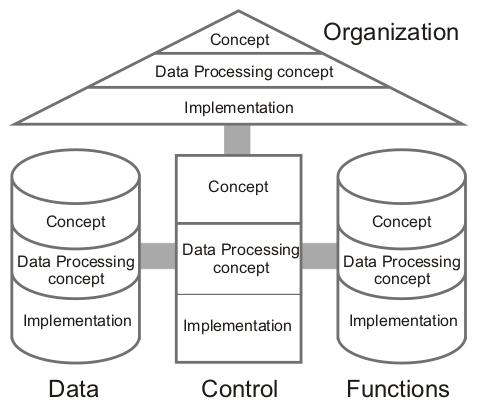
\includegraphics[width=0.8\textwidth]{aris}
				\caption{``allgemeiner Bezugsrahmen für Geschäftsprozessmodellierung.''}
			\end{figure}
			
			
			
			\subsubsection{Beschreibung der Sichten}
			
			\begin{tabularx}{\textwidth}{l|X|l}
				%\multicolumn{3}{c}{\textbf{Sichten}} \\[.5\normalbaselineskip]
				%\multicolumn{2}{c}{Modell ist stets Modell:} \\
				%\toprule
				\textbf{Sicht} & \textbf{Inhalt} & \textbf{Beispiel} \\
				\toprule
				\textbf{Datensicht} & beschreibt Informationsobjekte zu Repräsentation von Ereignissen und Zuständen. Auftrag ist abgewickelt & Auftrag ist abgewickelt \\[4\normalbaselineskip]
				\textbf{Funktionssicht} & beschreibt Funktionen und ihre Zusammenhänge in Form von Funktionsbäumen & (Teil)funktionen der Auftragsabwicklung \\[3\normalbaselineskip]
				\textbf{Organisationssicht} & beschreibt Struktur und Beziehungen und Aufgabenträgern und Organisationseinheiten & Herr M. Abt. Auftragsannahme \\[3\normalbaselineskip]
				\textbf{Steuerungssicht} & beschreibt die Verbindung zwischen den Sichten & Prozesskette: Auftragsabwicklung \\[0.5\normalbaselineskip]
				\bottomrule
			\end{tabularx}
			
			\bigskip
			%\\[2\normalbaselineskip]
			
			\subsubsection{Beschreibung der Schichten}
			\begin{tabularx}{\textwidth}{X|X|X}
				%\multicolumn{3}{c}{\textbf{Schichten}} \\[0.5\normalbaselineskip]
				%\toprule
				\textbf{Fachkonzept} & \textbf{DV-Konzept} & \textbf{Implementierung} \\
				\toprule
				\begin{itemize}[leftmargin=*]
					\item Anforderungsanalyse
					\item Darstellung fachlich-betriebswirtschaftlicher Sachverhalte
				\end{itemize}
				&
				\begin{itemize}[leftmargin=*]
					\item Anpassung des Fachkonzepts an die SOMETHING MISSING
					\item Anforderungen zur DV-technischen Unterstützung
				\end{itemize}
				&
				\begin{itemize}[leftmargin=*]
					\item Umsetzung in konkrete Soft- und Hardwarekomponenten
				\end{itemize}\\
				\bottomrule
			\end{tabularx}
			
			\bigskip
			%\hrulefill
			
			\subsubsection{EPK -- Steuerung: Fachkonzept}
			\begin{itemize}
				\item \textbf{Ereignis:} beschreibt eingetretenen Zustand
				\item \textbf{Funktion:} fachliche Aufgabe
				\item \textbf{Konnektoren:} AND ($\land$), XOR ($\otimes$), OR ($\lor$)
			\end{itemize}
			
			\pagebreak
			
			\subsection{Frage 2}
			\label{le4-2}
			\subsubsection{ERM -- Datensicht: Fachkonzept \& DV-Konzept \& Implementierung}
			\begin{itemize}
				\item \textbf{Entity:} Objekt der realen oder der Vorstellungswelt, über das Informationen zu speichern sind
				\item \textbf{Relation:} Beziehung zwischen Entities
				\item \textbf{Attribut:} Eigenschaft von Entities oder Beziehungen
			\end{itemize}
			
			\subsubsection{Modellierung des DV-Konzepts}
			\begin{itemize}
				\item Relationale Datenmodelle
				\begin{itemize}
					\item Chen-Notation -- 1:N
					\item Schlageter/Stucky-Notation -- N:1
					\item min, max Notation (0, *)
				\end{itemize}
				\item Objektorientierte Datenmodelle
			\end{itemize}
			
			\subsubsection{Implementierungsebene}
			\begin{itemize}
				\item Hardwareeinsatz
				\item Betrachtete Strukturen: Datenblöcke, Zeiger, Indexstrukturen
			\end{itemize}
			
			\hrulefill
			
			\subsubsection{Merkmal der Objektorientierung}
			\textbf{Objektorientierung:} Sichtweise auf komplexe Systeme, bei der ein System durch das Zusammenspiel kooperierender Objekte beschrieben wird um Komplexität zu reduzieren. \bigskip %\\[1\normalbaselineskip]
			
			
			\textbf{Objekt:} Abbildung eines realen oder imaginären Gegenstands
			\begin{itemize}
				\item Programmiertechnische Gegenstände (z.B. Button einer GUI)
				\item Gegenstände des Problembereichs (z.B. Bankkonto)
			\end{itemize} \bigskip
			
			\textbf{Objektorientierte Programmierung:}
			\begin{itemize}
				\item Ist ein Programmierparadigma, dass auf dem Konzept der Objektorientierung aufbaut
				\item Grundidee ist dabei Daten und Funktionen, die auf diese Daten angewendet werden können, in Objekten zusammenzufassen 
				\item Objekte verfügen dafür über einen Speicher (Attribute) und Funktionen (Methoden)
				\item Objekte integrieren miteinander durch das Senden von Nachrichten (gegenseitiges Aufrufen der Methoden)
			\end{itemize}
			
			\pagebreak
			
			\textbf{Klassen und Objekte}
			\begin{itemize}
				\item Eine Klasse ist die Definition der Attribute, Operationen und der Semantik für eine Menge von Objekten
				\item Ein Objekt ist ein Exemplar einer Klasse mit eigener Identität
				\begin{itemize}
					\item Der Zustand eines Objektes ist durch seine Attribute und Beziehungen zu anderen Objekten bestimmt
					\item Das Verhalten wird durch eine Menge Operationen/Methoden beschrieben. 
					\item Objekte kommunizieren Über Botschaften/Nachrichten. Eine Botschaft aktiviert eine Operation gleichen Namens. Ausgabedaten werden an den Sender der Botschaft zurückgegeben. Eine Änderung des Zustands eines Objektes erfolgt in der Regel über seine Operationen
				\end{itemize}
			\end{itemize}
			
			\subsection{Frage 3}
			\label{le4-3}
			\subsubsection{Wozu dient UML?}
			\begin{quote}
				Die \textbf{Unified Modeling Language}\footnote{UML bietet nur eine Notation, aber keine Methode, wie die Modellierung zu bewerkstelligen ist} ist eine graphische Sprache zur:
			\end{quote}
			
			\begin{itemize}
				\item Visualisierung
				\item Spezifikation
				\item Entwicklung
				\item Dokumentation der Artefakte softwareintensiver Systeme
			\end{itemize}
			
			\pagebreak
			
			\section{Lerneinheit 5}
			\subsection{Lernziele}
			\begin{enumerate}
				\item \hyperref[le5-1]{\textit{Sie verstehen den Nutzen von Modellen und kennen die allgemeinen Elemente der Modellierung.}}
				\item \hyperref[le5-2]{\textit{Sie kennen die Grundelemente von Geschäftsmodellen, des Business Model Canvas, der $E^3$ Value Methode sowie der Dienstleistungsmodellierung (Service Blueprint).}}
				\item \hyperref[le5-3]{\textit{Sie können betriebswirtschaftliche Sachverhalte in Geschäfts-, Wertfluss und Dienstleistungsmodellen darstellen.}}
			\end{enumerate}
			
			\subsection{Frage 1}
			\label{le5-1}
			\texttt{\hyperref[redir5-1--3-1]{WIRD BEREITS IN LERNEINHEIT 3 BESCHRIEBEN}}
			
			\subsection{Frage 2}
			\label{le5-2}
			\subsubsection{Geschäftsmodell}
			\begin{itemize}
				\item Abbildung des betrieblichen Produktions- und Leistungssystems eines Unternehmens
				\item sagt aus durch welche Kombination von Produktionsfaktoren die Geschäftsstrategie eines Unternehmens umgesetzt werden kann und welche Akteure was machen müssen
			\end{itemize}
			
			%\hrulefill doesn't fit the design -- only use hrulefill if we start a new subsection that still answers the same question
			
			
			\subsubsection{Elemente eines Geschäftsmodells}
			\begin{itemize}
				\item \textbf{Wer} sind die Zielkunden? --- Der \textbf{Kunde}
				\item \textbf{Was} bieten wir den Kunden? --- Der \textbf{Wertbeitrag}
				\item \textbf{Wie} entsteht ein Wertfluss? --- Der \textbf{Wertfluss}
				\item \textbf{Warum} wird Gewinn erzielt? --- Der \textbf{Gewinn}
			\end{itemize}
			
			\subsubsection{Geschäftsmodellinovation}
			
			\begin{quote}
				...schafft neue Logik hinsichtlich wie das Unternehmen einen Wert schafft, indem es Änderungen an den obigen Fragen vornimmt.
			\end{quote}
			\bigskip
			
			\textbf{Beispiele:}
			\begin{itemize}
				\item Neuerfindungen 
				\item Ersatz bestehender Produkte und Services 
				\item Schaffung neuer digitaler Geschäftsmodelle
			\end{itemize}
			
			\hrulefill
			
			\subsubsection{Canvas Elemente}
			\begin{figure}[H]
				\centering
				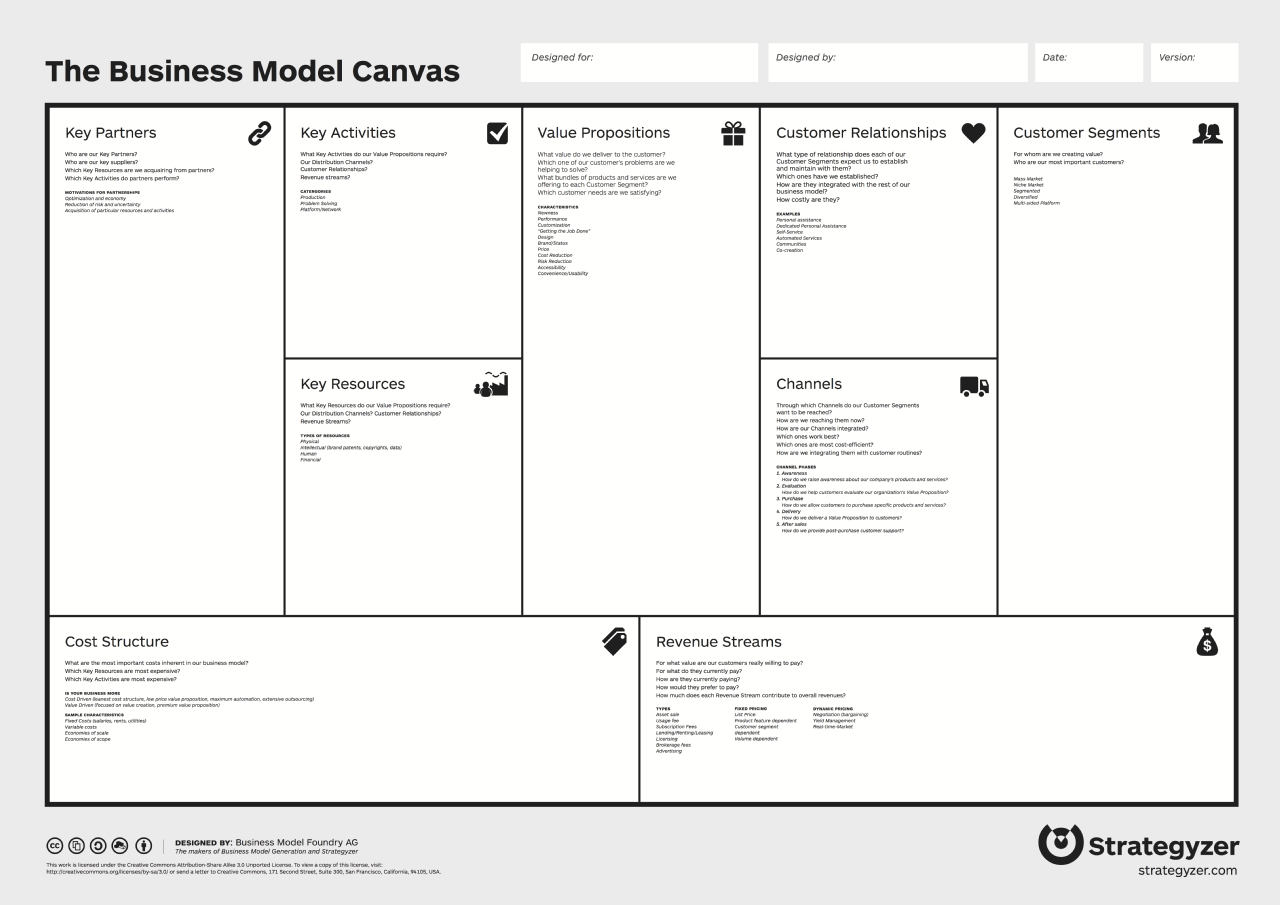
\includegraphics[width=1\textwidth]{canvas}
				\caption{Das Business Model Canvas}
			\end{figure}
			
			\begin{enumerate}
				\item key \textbf{p}artners 
				\item key \textbf{a}ctivities 
				\item key \textbf{r}esource 
				\item channels
				\item customer relationships $<$3
				\item customer segments 
				\item cost structure 
				\item revenue streams 
				\item value proposition
			\end{enumerate}
			
			\hrulefill
			
			\pagebreak
			
			\subsubsection{ \textnormal{$e^3$} Value Method} %shit doesn't even change anything wtf
			Modellierung von Wertflüssen zwischen Akteuren. Fokus: Austausch von Wertobjekten
			
			\subsubsection{Elemente}
			\begin{itemize}
				\item Akteur: unabhängige wirtschaftliche Einheit 
				\item Marktsegment: Menge von Akteuren mit gleichen Wertobjekten und -Schnittstellen 
				\item Wertobjekt: Austauschobjekt zwischen Akteuren, das einen Wert darstellt 
				\item Wertkanal: Angebots-/Nachfrageindikator für Wertobjekte 
				\item Wertschnittstelle: Fasst Wertkanäle zusammen und zeigt an, was wofür ausgetauscht wird 
				\item Wertaustausch: Verbindung zweier Wertkanäle Austauschbeziehungen 
				\item Szenario Pfad: Beschreibt den Wertfluss einer Transaktion des Modells 
				\item Start-/Stoppstimulus: Anfang und Ende des Szenario Pfads
			\end{itemize}
			
			\hrulefill
			
			\subsubsection{Service Blueprint}
			Methode zur Modellierung von Dienstleistungsprozesse und Grundlager zur Innovationen Unterscheidet Dienstleistungsprozesse hinsichtlich der Kundeninteraktion, Kundenwarnehmung und internen Prozessen.
			
			\subsubsection{Linien und Ebenen im Service Blueprint}
			\begin{itemize}
				\item interaction 
				\item visibilitiy 
				\item internal interaction 
				\item order penetration 
				\item implementation
			\end{itemize}
			
			
			
			\subsection{Frage 3}
			\label{le5-3}
			\texttt{Wird hier nicht beantwortet - am liebsten die ganze Frage wegstreichen}
			
			\pagebreak
			
			\section{Lerneinheit 6}
			\subsection{Lernziele}
			\begin{enumerate}
				\item \hyperref[le6-1]{\textit{Sie kennen branchenneutrale Anwendungssysteme im Überblick.}}
				\item \hyperref[le6-2]{\textit{Sie kennen dabei die wichtigsten der von ihnen unterstützten Teilprozesse und Entitäten.}}
				\item \hyperref[le6-3]{\textit{Sie sind mit den verschiedenen Arten von Führungsinformationssystemen vertraut.}}
			\end{enumerate}
			
			\subsection{Frage 1}
			%	\subsubsection{Enterprise Resource Planning (ERP)\footnote{Zusammen mit einer zentralen Datenbasis verbunden}}
			\subsubsection{Enterprise Resource Planning (ERP)\footnote{Zusammen mit einer zentralen Datenbasis verbunden}}
			\begin{itemize}
				\item Vertrieb Marketing
				\item Personalwesen
				\item Produktion
				\item Finanz und Rechnungswesen
			\end{itemize}
			
			\subsection{Frage 2}
			\subsubsection{Prozessmodell}
			\begin{quote}
				Informations- und Dispositionsprozesse $\rightarrow$ \textbf{Steuerung des Unternehmens} \\
				Leistungserstellungsprozesse $\rightarrow$ \textbf{Leistungserbringung am Markt} \\
				Administrationsprozesse $\rightarrow$ \textbf{Dokument und Verwaltung}
			\end{quote}
			\bigskip
			\hrulefill
			
			\subsubsection{Klassifikation der Führungsunterstützungssysteme}
			\bigskip
			\begin{tabularx}{\textwidth}{X|X|X}
				\multicolumn{3}{c}{\textbf{I GOTTA FIGURE OUT A PROPER LAYOUT FOR THIS SHIT}} \\[1\normalbaselineskip]
				\multicolumn{3}{c}{\textbf{Führungsinformationssysteme}} \\[1\normalbaselineskip]
				\textbf{Führungsinformationssysteme} & \textbf{Klassifikation} & \textbf{Ziel} \\
				\toprule
				\textbf{Informationssysteme} & moo & \textbf{asd} \\
				\midrule
				\textbf{Führrungssysteme} & \textbf{} & \textbf{} \\
				\bottomrule
				
				
				
				
			\end{tabularx}
			
			\bigskip
			
			\begin{tabular}{m{5cm} c}
				\hline
				\begin{verbatim}
				sudo apt update
				ldskjfdslkjf
				sfds
				\end{verbatim}
				& description
				\\ \hline
			\end{tabular}
		
		
		
		
	\end{document}